\section{}
\paragraph{}\label{answer:35}
مسأله این است که ما یک متغیر محلی به نام \lr{\texttt{remove}} تعریف کردیم. یک تابع استاندارد به نام \lr{\texttt{remove}} نیز وجود دارد. متغیر محلی ما، این تابع را در حوزهٔ متغیر محلی، پوشاند. این حوزه در پایان اولین \lr{\texttt{if}} در خط 15 به پایان رسید. عبارت بعدی یعنی \lr{\texttt{16   if (remove)}} بررسی می‌کند که آیا آدرس تابع \lr{\texttt{remove}} غیرصفر است یا نه و اگر باشد، عبارت بعدی را اجرا می‌کند.

\begin{center}
    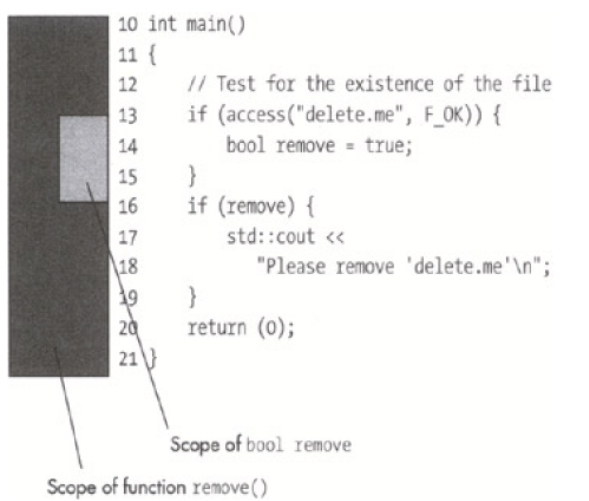
\includegraphics[keepaspectratio,width=0.4\textwidth,height=0.4\textheight]{images/image02.jpg}
\end{center}